\documentclass[12pt]{article}
\usepackage[english]{babel}
\usepackage[utf8]{inputenc}

%% Pointer to 'default' preamble
% pacakages and definitions

\usepackage{geometry}
\geometry{
	letterpaper, 
	portrait, 
	top=.75in,
	left=.8in,
	right=.75in,
	bottom=.5in		} 	% Page Margins
	
%% additional packages for nice things
\usepackage{amsmath} 	% for most math
\usepackage{commath} 	% for abs
\usepackage{lastpage}	% for page count
\usepackage{amssymb} 	% for therefore
\usepackage{graphicx} 	% for image handling
\usepackage{wrapfig} 	% wrap figures
\usepackage[none]{hyphenat} % for no hyphenations
\usepackage{array} 		% for >{} column characterisctis
\usepackage{physics} 	% for easier derivative \dv....
\usepackage{tikz} 		% for graphic@!
\usepackage{circuitikz} % for circuits!
\usetikzlibrary{arrows.meta} % for loads
\usepackage[thicklines]{cancel}	% for cancels
\usepackage{xcolor}		% for color cancels
\usepackage[per-mode=fraction]{siunitx} % for si units and num
\sisetup{group-separator = {,}, group-minimum-digits = 3} % additional si unit table functionality

\usepackage{fancyhdr} 	% for header
\usepackage{comment}	% for ability to comment out large sections
\usepackage{multicol}	% for multiple columns using multicols
\usepackage[framed,numbered]{matlab-prettifier} % matlab sytle listing
\usepackage{marvosym} 	% for boltsymbol lightning
\usepackage{pdflscape} 	% for various landscape pages in portrait docs.
%\usepackage{float}
\usepackage{fancyvrb}	% for Verbatim (a tab respecting verbatim)
\usepackage{enumitem}	% for [resume] functionality of enumerate
\usepackage{spreadtab} 	% for using formulas in tables}
\usepackage{numprint}	% for number format in spread tab
\usepackage{subcaption} % for subfigures with captions
\usepackage[normalem]{ulem} % for strike through sout

% for row colors in tables....
\usepackage{color, colortbl}
\definecolor{G1}{gray}{0.9}
\definecolor{G2}{rgb}{1,0.88,1}%{gray}{0.6}
\definecolor{G3}{rgb}{0.88,1,1}

% For table formatting
\usepackage{booktabs}
\renewcommand{\arraystretch}{1.2}
\usepackage{floatrow}
\floatsetup[table]{capposition=top} % put table captions on top of tables

% Caption formating footnotesize ~ 10 pt in a 12 pt document
\usepackage[font={small}]{caption}

%% package config 
\sisetup{output-exponent-marker=\ensuremath{\mathrm{E}}} % for engineer E
\renewcommand{\CancelColor}{\color{red}}	% for color cancels
\lstset{aboveskip=2pt,belowskip=2pt} % for more compact table
%\arraycolsep=1.4pt\def
\setlength{\parindent}{0cm} % Remove indentation from paragraphs
\setlength{\columnsep}{0.5cm}
\lstset{
	style      = Matlab-editor,
	basicstyle = \ttfamily\footnotesize, % if you want to use Courier - not really used?
}
\renewcommand*{\pd}[3][]{\ensuremath{\dfrac{\partial^{#1} #2}{\partial #3}}} % for larger pd fracs
\renewcommand{\real}[1]{\mathbb{R}\left\{ #1 \right\}}	% for REAL symbol
\newcommand{\imag}[1]{\mathbb{I}\left\{ #1 \right\}}	% for IMAG symbol
\definecolor{m}{rgb}{1,0,1}	% for MATLAB matching magenta
	
%% custom macros
\newcommand\numberthis{\addtocounter{equation}{1}\tag{\theequation}} % for simple \numberthis command

\newcommand{\equal}{=} % so circuitikz can have an = in the labels
\newcolumntype{L}[1]{>{\raggedright\let\newline\\\arraybackslash\hspace{0pt}}m{#1}}
\newcolumntype{C}[1]{>{\centering\let\newline\\\arraybackslash\hspace{0pt}}m{#1}}
\newcolumntype{R}[1]{>{\raggedleft\let\newline\\\arraybackslash\hspace{0pt}}m{#1}}

%% Header
\pagestyle{fancy} % for header stuffs
\fancyhf{}
% spacing
\headheight 29 pt
\headsep 6 pt

%% Header
\rhead{Thad Haines \\ Page \thepage\ of \pageref{LastPage}}
\chead{Mini WECC \\   10 Minute AGC Recovery (Generator Trips 02)}
\lhead{Research \\ 08/20/20}

\usepackage[hidelinks]{hyperref} % allow links in pdf
\usepackage{setspace}
\usepackage{multicol}
%\usepackage{minted}

\begin{document}
\onehalfspacing
\paragraph{10 Minute AGC Recovery of Mini WECC after 2 Generator Trips} \ \\

\begin{minipage}{0.5\linewidth}
\begin{itemize}
\raggedright
%\item Mini WECC system:
%\begin{itemize}
%\itemsep 0 em
%\small
%\item Buses: 122
%\item Lines: 171
%\item Loads: 88
%\item Machines: 34
%\item States: 623
%\end{itemize}
\item Events: Trip of Bus 1 Gen at t= 5\\ Trip of Bus 30 Gen at t = 8

\item Each area has identical conditional AGC that acts at t=40 and again when t=160, 280, 400, 520 (i.e. 2 minute action time).

\item ODE solver tolerances:
\subitem Relative: 1e-5
\subitem Absolute: 1e-7

\item States and derivatives of tripped machines set to zero.

\end{itemize}
\vfill
\end{minipage}\hspace{2em}% 
\begin{minipage}{0.4\linewidth}
\centering
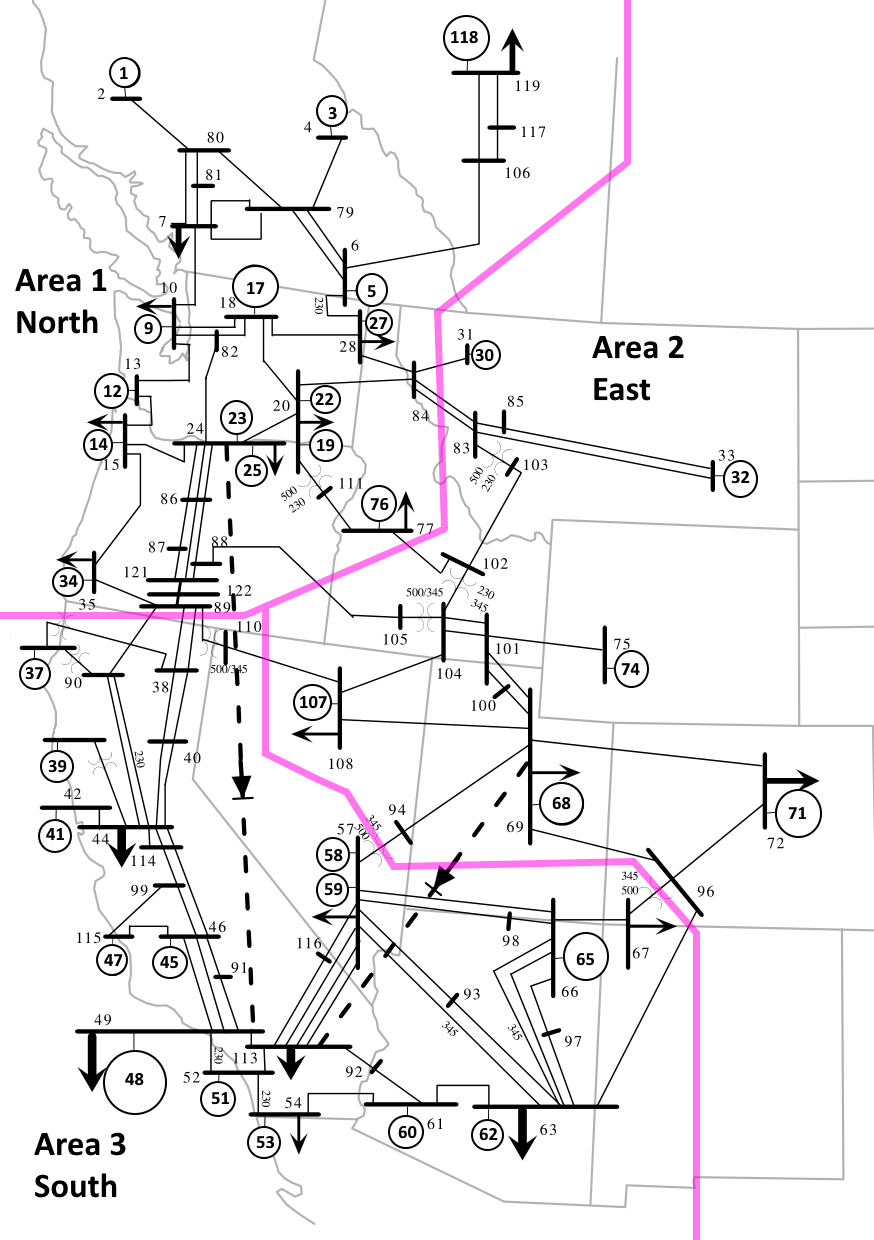
\includegraphics[width=.8\linewidth]{miniWECC_split03.png}
\end{minipage}% 


\begin{table}[!ht]
\resizebox{\linewidth}{!}{
	\centering
	\begin{tabular}{@{} L{2.5cm} 
	R{2cm} R{2cm}  R{2cm} R{1.5cm} R{0.75cm} R{0.75cm} R{1.5cm} R{2cm} R{2cm}@{}} 	
		\toprule % @ signs to remove extra L R space
		\footnotesize % this will affect the table font (makse it 10pt)
		\raggedright % for non justified table text

	&	\multicolumn{3}{c}{Step Size [seconds]}					&		&	\multicolumn{2}{c}{\shortstack{Solutions\\Per Step}}			&		&		&		\\
Method	&	Max.	&	Min.	&	Ave.	&	Total Steps	&	Ave.	&	Max.	&	\shortstack{Total\\Slns.}	&	Sim. Time	&	Speed Up	\\ \midrule
FTS	&	0.0083	&	8.30E-04	&	0.0083	&	72,001	&	2	&	2	&	144,002	&	707.51	&	1.00	\\
VTS	&	0.5333	&	2.03E-06	&	0.0273	&	22,006	&	3	&	783	&	57,448	&	540.02	&	1.31	\\
VTS - 0dx	&	3.2744	&	2.03E-06	&	0.0757	&	7,932	&	3	&	781	&	21,260	&	210.51	&	3.36	\\
																			\bottomrule



	\end{tabular}
	}%end resize box
\end{table}

\paragraph{Result Summary:}
\begin{itemize}
\item Zeroing out of machine states and derivatives decreased required simulation time.
\item Unsure why time steps remained `small' when $t>300$.
\end{itemize}

\begin{center}
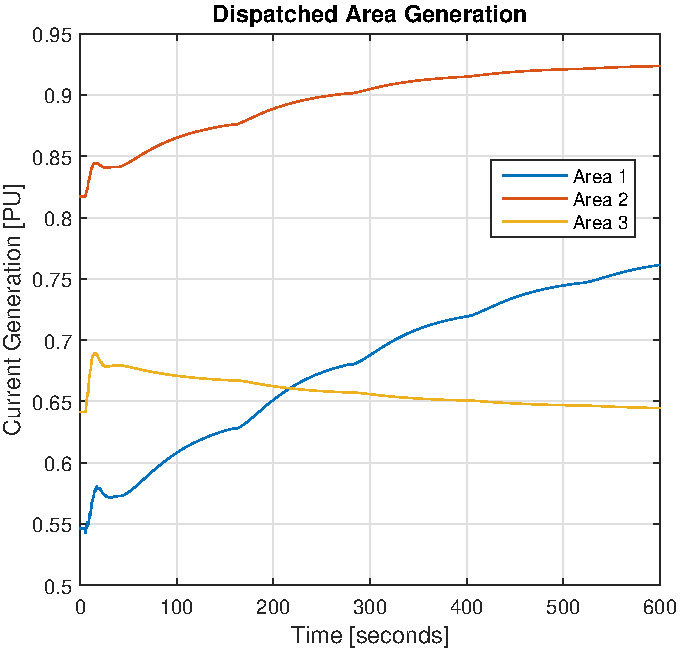
\includegraphics[width=.45\linewidth]{AGCdisp}%
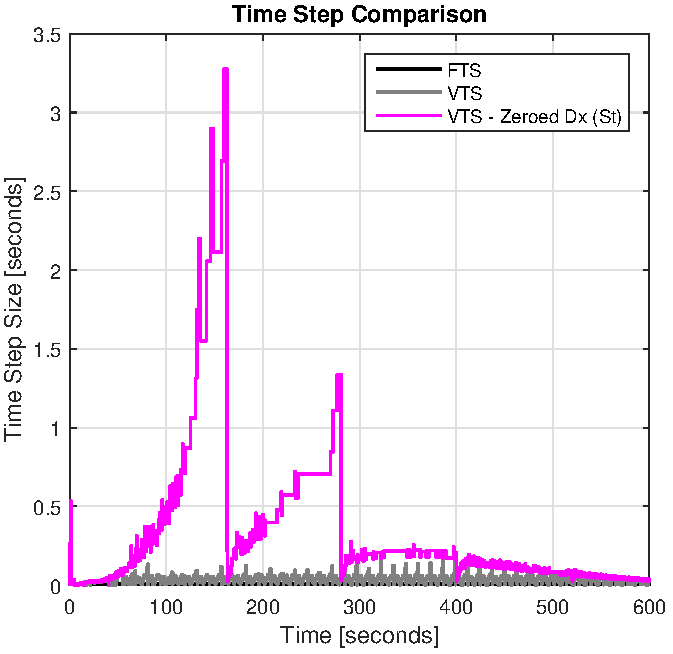
\includegraphics[width=.45\linewidth]{tripStepSz}%
\end{center}



\end{document}
